\documentclass[preview]{standalone}

\usepackage{amsmath}
\usepackage{amssymb}
\usepackage{stellar}
\usepackage{definitions}
\usepackage{bettelini}
\usepackage{tikz}

\begin{document}

\id{mechanics-ex-4}
\genpage

\section{Exercises - Batch 4}

\begin{snippetexercise}{mechanics-ex-4.1}{\underline{4.1}}
    Two bodies, \(A\) and \(B\), with respective masses \(M_A\) and \(M_B\),
    where \(M_B>M_A\), slide down an inclined plane (with an inclination angle \(\alpha\)).
    They are in contact with each other,
    with \(B\) positioned higher than \(A\).
    Calculate the acceleration of the system consisting of the two bodies, if the coefficients of friction
    are \(\mu_A\) and \(\mu_B\) respectively. With what force does body \(B\) push body \(A\)?
\end{snippetexercise}

\begin{snippetsolution}{mechanics-ex-4.1-sol}{\underline{4.1}}
    \todo
\end{snippetsolution}

\begin{snippetexercise}{mechanics-ex-4.2}{\underline{4.2}}
    A rope passing over a frictionless pulley has two masses, \(M\) and \(m\), attached at its ends,
    with \(M>m\). Determine the acceleration of the system and the tension in the rope.
\end{snippetexercise}

\begin{snippetsolution}{mechanics-ex-4.2-sol}{\underline{4.2}}
    \todo
\end{snippetsolution}

\begin{snippetexercise}{mechanics-ex-4.3}{\underline{4.3}}
    Assuming all surfaces are frictionless and the inertia of the rope and pulley is negligible,
    find the value of the horizontal force \(F\) such that there is no relative motion between
    the masses \(m_1\), \(m_2\), and \(M\)\\
    \begin{center}
        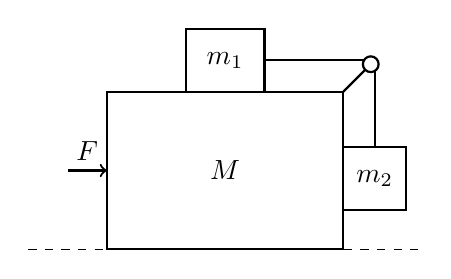
\begin{tikzpicture}
            % Draw ground line
            \draw[dashed] (-1,0) -- (4,0);
        
            % Draw the large block M
            \draw[thick] (0,0) rectangle (3,2);
            \node at (1.5,1) {$M$};
        
            % Draw the force vector F
            \draw[thick, ->] (-0.5,1) -- (0,1) node[midway, above] {$F$};
        
            % Draw the small block m1 on top of M
            \draw[thick] (1,2) rectangle (2,2.8);
            \node at (1.5,2.4) {$m_1$};
        
            % Draw the small block m2 on the right of M
            \draw[thick] (3,0.5) rectangle (3.8,1.3);
            \node at (3.4,0.9) {$m_2$};
        
            % Draw the pulley system
            \draw[thick] (2,2.4) -- (3.4,2.4) -- (3.4,1.3);
            \draw[thick] (3,2) -- (3.35,2.35);
            \draw[thick, fill=white] (3.35,2.35) circle(0.1);
        \end{tikzpicture}
    \end{center}
\end{snippetexercise}

\begin{snippetsolution}{mechanics-ex-4.3-sol}{\underline{4.3}}
    \todo
\end{snippetsolution}

\begin{snippetexercise}{mechanics-ex-4.4}{\underline{4.4}}
    A particle of mass \(m\) is constrained to move without friction inside a conical
    surface with an angle \(\alpha\).
    Find the initial conditions such that the particle moves
    in uniform circular motion relative to the vertical axis of the cone.
\end{snippetexercise}

\begin{snippetsolution}{mechanics-ex-4.4-sol}{\underline{4.4}}
    \todo
\end{snippetsolution}

\begin{snippetexercise}{mechanics-ex-4.5}{\underline{4.5}}
    A block of mass \(m_1\) is placed on top of a block of mass \(m_2\), which is at rest on a smooth floor.
    If the coefficient of friction between the two blocks is \(\mu\), find the maximum value of the horizontal
    force FF that can be applied to \(m_2\) so that \(m_1\) does not slip.
\end{snippetexercise}

\begin{snippetsolution}{mechanics-ex-4.5-sol}{\underline{4.5}}
    \todo
\end{snippetsolution}

\begin{snippetexercise}{mechanics-ex-4.6}{\underline{4.6}}
    A body of mass \(m\), placed on a rough horizontal plane (friction coefficient \(\mu\)),
    is pulled by a force \(F\) forming an angle \(\alpha\) with the horizontal.
    The body moves at a constant velocity.
    Determine the angle \(\alpha\) for which the force intensity is minimal;
    also, calculate the value of this minimal force.
\end{snippetexercise}

\begin{snippetsolution}{mechanics-ex-4.6-sol}{\underline{4.6}}
    \todo
\end{snippetsolution}

\begin{snippetexercise}{mechanics-ex-4.7}{\underline{4.7}}
    Two blocks, \(A\) and \(B\), with respective masses \(m_A\) and \(m_B\),
    are connected by a massless inextensible rope.
    Block \(A\) rests on an inclined plane with an angle \(\alpha\) relative to the horizontal
    and is also attached to a spring with elastic constant \(k\), whose other end is fixed to a support
    at the base of the inclined plane. Block \(B\) hangs through a pulley parallel to the vertical
    leg of the triangle formed by the inclined plane. Neglecting friction, determine the oscillation period of the
    two bodies around the equilibrium position.
\end{snippetexercise}

\begin{snippetsolution}{mechanics-ex-4.7-sol}{\underline{4.7}}
    \todo
\end{snippetsolution}

\end{document}